\chapter{Metodologia}

A metodologia é esquematizada na figura \ref{fig:metodologia} que ilustra o fluxo de trabalho. Esse processo envolve a definição do problema,
a escolha do banco, o pré-processamento, escolha das estratégias de validação, e aplicação do modelo, culminando na escolha do melhor modelo.

\begin{figure}[H]
  \centering
  \caption{Esquema a metodologia adotada.}
  \begin{tikzpicture}[node distance=1.5cm, every node/.style={draw, rounded corners, minimum width=2.8cm, minimum height=1cm, align=center}]

%passos
\node (passo0) {Definição do problema};
\node [below=of passo0] (passo1) {Escolha do banco};
\node [below=of passo1] (passo2) {Pré processamento};
\node [below=of passo2] (passo3) {Escolha dos modelos};
\node [below=of passo3] (passo4) {Escolha da estratégia de validação};
\node [below=of passo4] (passo5) {Aplicação do modelo};
\node [below=of passo5] (passo6) {Escolha do melhor modelo};

%conexões
\draw[->](passo0) -- (passo1);
\draw[->](passo1) -- (passo2);
\draw[->](passo2) -- (passo3);
\draw[->](passo3) -- (passo4);
\draw[->](passo4) -- (passo5);
\draw[->](passo5) -- (passo6);

\end{tikzpicture} % insere o tikzpicture puro
  \label{fig:metodologia}
  \legend{Fonte: Elaborado pelo autor.}
\end{figure}

Cada um desses passos introduz considerações, e as decisões tomadas influenciam nos passos seguintes. Por exemplo, a escolha do banco impacta diretamente em 
quais tipos de pré-processamento necessário, como a limpeza. Contanto, antes mesmo da escolha do banco, é necessário definir qual o problema, visto que 
que as anotações presentes podem limitar o escopo dos problemas resolvidos. 

Nas seções subsequentes, detalha-se as decisões adotadas em cada etapa da metodologia, bem como os critérios considerados para tais escolha


\section{O banco de dados}
\label{sec:particionamento}

Optou-se pelo \textit{MIT-BIH Arrhythmia Database} \cite{mitbih2005}. Segundo \citeonline{physionet_annotations}, o banco é composto por 58 registros de eletrocardiograma (ECG), cada um com 30 minutos de duração. 
Os 23 primeiros registros, de 100 a 124, foram selecionados aleatoriamente a partir de um conjunto de 4000 gravações de 24 horas realizadas em pacientes ambulatoriais do Beth Israel Deaconess Medical Center. 
Os 25 registros, 200 até 234, restantes foram escolhidos de modo a incluir arritmias raras e com formato complexo, mas clinicamente significativas.
Cada uma das anotações foram feitas com por três cardiologistas independentes. Os sinais foram coletados com duas derivações; uma superior e outra inferior. A superior
é majoritariamente utilizando a derivação MLII (modified limb II) que é feita com o eletrodo no peito. 
Em alguns casos, foi utilizado as derivações V1 (ou mais raramente, V2, V3 e V4); que também são obtidas com os eletrodos no peito.

Neste trabalho, foi utilizado somente a derivação superior, pois permite uma melhor visão do complexo QRS \cite{physionet_annotations}.

Na tabela \ref{tab:mapeamento_classes}, é detalhado o mapeamento entre as classes originais de batimentos para as cinco definidas pela AAMI.

\begin{table}[H]
\centering
\caption{Mapeamento das anotações originais do MIT-BIH para as classes AAMI.}
\label{tab:mapeamento_classes}
\begin{tabular}{ll}
\hline
\textbf{Anotação Original} & \textbf{Classe AAMI} \\
\hline
N, e, j, L, R & N (Normal) \\
A, a, J, S & S (Supraventricular) \\
V, E & V (Ventricular) \\
F, f & F (Fusão) \\
Q, ?, / & Q (Desconhecida) \\
\hline
\end{tabular}
\legend{Fonte: Adaptado de Silva et al. (2025).}
\end{table}

O objetivo foi a detecção de batimentos da classe V que compreende: contração prematura ventricular (ou PVC, classe V) e batimento ventricular de escape, classe E, \cite{physionet_annotations}.
Conforme discutido na seção \ref{sub_sec:padroes_arritmias_aami}, apesar de ocorrerem em indivíduos saudáveis, esses tipos arrítmicos possuem relevância clínica pois estão associados a tipos mais graves.

Essas anotações são anotações de batimento, isto é, elas são feitas em cada pico R no ECG. Além delas, existem as anotações de ritmo dentro as quais, podemos destacar: o ritmo normal identificado por (N,
e a taquicardia ventricular; identificado por (VFL.

O MIT-BIH é um banco aberto e muito utilizado para a classificação de arritmias, permitindo uma comparação com demais trabalhos.
Além de ser recomendado pela AAMI.

\section{Pré-processamento}
\label{sec:pre_process}

Antes de usar o sinal do ECG como entrada, ele precisou passar por uma etapa de pré-processamento que consistiu em uma limpeza de ruídos e segmentação.
Para a diminuição do ruído, foi utilizando um filtro passa-alta de ordem 5 de 0,5 hz, seguido por uma filtragem de linha de energia de 60hz. 
Isso foi importante para remover ruídos musculares e ruídos oriundos da alimentação dos aparelhos. 

Em seguida, os batimentos foram segmentados em batimentos individuais. Nas duas etapas foram utilizadas a biblioteca NeuroKit2 \cite{Makowski2021neurokit}

\subsection{Features}

A única \textit{feature} usada foi o intervalo RR que é calculado da seguinte forma: 

\begin{equation}
\text{pré RR intervalo} = R_{i-1} - R_{i}
\end{equation}

\begin{equation}
\text{pós RR intervalo} = R_{i} - R_{i+1}
\end{equation}

Esses intervalos correspondem ao intervalo entre o batimento \textit{i} e o anterior e posterior, respectivamente.

\section{Arquiteturas}
\label{sec:modelos}

Foram testadas dois tipos de arquiteturas, uma é o uso de RNNs puras e a outra é uma arquitetura híbrida com CNNs. 

A primeira arquitetura de pura é composta por três camadas de GRUs com 256 unidades ocultas. Essa arquitetura foi utilizada em \citeonline{narotamo2024}, onde obteve o melhor desempenho. 
A diferença é que nesse trabalho, além da rede receber o sinal do ECG, ela também recebeu os intervalos RRs pré e pós:


\begin{figure}[H]
  \centering
  \caption{Arquitetura GRU pura.}
  \begin{tikzpicture}[node distance=1.5cm, every node/.style={draw, rounded corners, minimum width=2.8cm, minimum height=1cm, align=center}]

\node (input){Entrada ECG e features};
\node [below=of input](gru_1){GRU};
\node [below=of gru_1](gru_2){GRU};
\node [below=of gru_2](gru_3){GRU};
\node [below=of gru_3](saida){Classificação final};

%conexões:

\draw[->](input) -- (gru_1);
\draw[->](gru_1) -- (gru_2);
\draw[->](gru_2) -- (gru_3);
\draw[->](gru_3) -- (saida);
\end{tikzpicture}
 % insere o tikzpicture puro
  \label{fig:gru_pura}
  \legend{Fonte: Elaborado pelo autor.}
\end{figure}

A segunda rede é uma híbrida de CNN com GRU:

\begin{figure}[H]
  \centering
  \caption{Arquitetura híbrida CNN e GRU.}
  \begin{tikzpicture}[node distance=1.5cm, every node/.style={draw, rounded corners, minimum width=2.8cm, minimum height=1cm, align=center}]

% Entradas
\node (morf) {Entrada Morfológica (ECG)};
\node[right=of morf] (ritmo) {Entrada features};

%blocos de redes neurais:
\node[below=1.5cm of morf] (cnn) {Bloco CNN \\ (extração morfológica)};

% Combinação
\node[below=1.5cm of cnn, xshift=2.5cm] (fusion) {Combinação das Saídas};

% Bloco RNN
\node[below=of fusion] (rnn) {Bloco GRU \\ (padrões temporais)};

%saída
\node[below=of rnn] (saida) {Classificação Final};

%conexões
\draw[->](morf) -- (cnn);
\draw[->](cnn) -- ++ (fusion);
\draw[->](ritmo) -- ++ (fusion);
\draw[->](fusion) -- (rnn);
\draw[->](rnn) -- (saida);

\end{tikzpicture}

 % insere o tikzpicture puro
  \label{fig:cnn_gru}
  \legend{Fonte: Elaborado pelo autor.}
\end{figure}

O bloco de CNN precisou ser aplicado em cada batimento dentro da sequência. Trata-se de duas camadas de CNN com 32 e 64 filtros respectivamente e cada 
uma seguida por uma camada de \textit{batch normalization} e \textit{global max pooling} para evitar sobre ajuste e reduzir as \textit{features} respectivamente.

Enquanto que a rede da figura \ref{fig:gru_pura} recebeu o ECG concatenado com as \textit{features}, a rede híbrida as recebeu separadas, sendo conectadas após o processamento
das CNNs.

Ambos os modelos recebem uma sequência de 16 batimentos junto com as \textit{features} RR.

Para otimização do processo de treinamento, foram utilizados os mecanismos de \textit{early stopping} e \textit{reduce on plateau}, responsáveis por limitar o número de épocas e ajustar dinamicamente a taxa de aprendizagem, respectivamente.

\section{Estratégia de avaliação}

Os dados foram particionados seguindo a estratégia inter-paciente proposta por Chazel et al. (apud \citeonline{silva2025}), na qual batimentos de um mesmo paciente não podem aparecer simultaneamente nos conjuntos de treinamento e validação. 
O objetivo é garantir a capacidade de generalização do modelo para diferentes pacientes. 
Além disso, conforme recomendado pela AAMI, registros de pacientes com marcapasso foram excluídos.

Nesta divisão, o banco costuma ser dividido em Ds1 e Ds2. O primeiro costuma ser usado para treino e o segundo para teste.
Os registros 101, 106, 108, 109, 112, 114, 115, 116, 118, 119, 122, 124, 201, 203, 205, 207, 208, 209, 215, 220, 223 e 230 formam o DS1. Os demais (100, 103, 105, 111, 113, 117, 121, 123, 200, 202, 210, 212, 213, 214, 219, 221, 222, 228, 231, 232, 233 e 234), o Ds2

Note que o conjunto Ds1 inclui 12 registros que são resultados da seleção aleatória e 22 dos registros com as morfologias complexas. Já no Ds2 possui 
oito dessa primeira seleção e 22 da segunda; sendo mais desafiador e feito para testar a capacidade de generalização do modelo.

Na tabela \ref{tab:particionamento}, é mostrado a distribuição das cinco classes nos dois conjuntos.

\begin{table}[htb]
\centering
\caption{Particionamento inter-paciente proposto por Chazel et al.}
\label{tab:particionamento}
\begin{tabular}{|l|c|c|c|c|c|c|}
\hline
Conjunto & N & SVEB & VEB & F & Q & Total \\ \hline
DS1 & 45 866 & 944 & 3 788 & 415 & 8 & 51 021 \\ \hline
DS2 & 44 259 & 1 837 & 3 221 & 388 & 7 & 49 712 \\ \hline
Total & 90 125 & 2 781 & 7 009 & 803 & 15 & 100 733 \\ \hline
\end{tabular}
\legend{Fonte: Adaptado de Silva et al. (2025).}
\end{table}

Como pode ser observado, as classes são desbalanceadas dentro do mesmo conjunto, porém, balanceada entre eles.

A avaliação foi feita utilizando uma avaliação cruzada no conjunto Ds1 inicialmente com duas partições (dois \textit{folds}) e, posteriormente, com cinco partições (cinco \textit{folds}) nos modelos finais, utilizando o particionados
inter-paciente. Esta estratégia permite avaliar o modelo com ECGs de pacientes para o qual ele não foi treinado; sendo mais próximo de um contexto clínico 
e expõe o modelo a mais variação.

Outra estratégia ser o particionamento intra-paciente, onde batimentos de um mesmo paciente podem aparecer tanto no treino quanto na validação. Essa estratégia seria 
mais adequada para um modelo personalizado, por exemplo. 

\subsection{Métricas}
\label{sec:metricas}

As métricas utilizadas para avaliar o desempenho dos modelos foram: sensibilidade, precisão, acurácia, \textit{F1-score}, AUC (\textit{Area Under the Curve}) e AP (textit{Average Precision}). Esses 
dois últimos são exibidos juntos ao gráficos \textit{ROC} e \textit{PR}, respectivamente.

A sensibilidade representa a capacidade do modelo em identificar corretamente as classes positivas, isto é, os batimentos arrítmicos. Sua equação é dada por:

\begin{equation}
\text{Sensibilidade} = \frac{TP}{TP + FN}
\end{equation}

em que $TP$ são os verdadeiros positivos e $FN$ os falsos negativos.  

A precisão, por sua vez, indica a proporção de batimentos classificados como arrítmicos que realmente pertencem a essa classe:

\begin{equation}
\text{Precisão} = \frac{TP}{TP + FP}
\end{equation}

onde $FP$ representa os falsos positivos. Precisão e sensibilidade estão relacionadas por um \textit{trade-off}. No contexto médico, prioriza-se elevada sensibilidade, ainda que à custa de menor precisão, uma vez que falsos negativos são mais prejudiciais que falsos positivos.  

O \textit{F1-score} é a média harmônica entre precisão e sensibilidade, buscando um equilíbrio entre ambas:

\begin{equation}
\text{\textit{F1-score}} = \frac{2 \cdot \text{Precisão} \cdot \text{Sensibilidade}}{\text{Precisão} + \text{Sensibilidade}}
\end{equation}

A acurácia corresponde ao acerto global do modelo, considerando tanto as classes positivas quanto as negativas:

\begin{equation}
\text{Acurácia} = \frac{TP + TN}{TP + TN + FP + FN}
\end{equation}

A AUC mede a capacidade do modelo em separar as classes positivas das negativas, variando entre 0 e 1. Valores próximos de 1 indicam separação perfeita, enquanto 0,5 corresponde a um modelo com desempenho equivalente ao acaso,
o \textit{baseline}.

Essa métrica é calculada a partir da área sob a curva ROC. Na Figura~\ref{fig:roc_perfect}, é ilustrado a curva ROC de um classificador perfeito.

\begin{figure}[H]
    \centering
    \caption{Curva ROC de um Classificador Perfeito: Comparação com Modelo Aleatório.}
    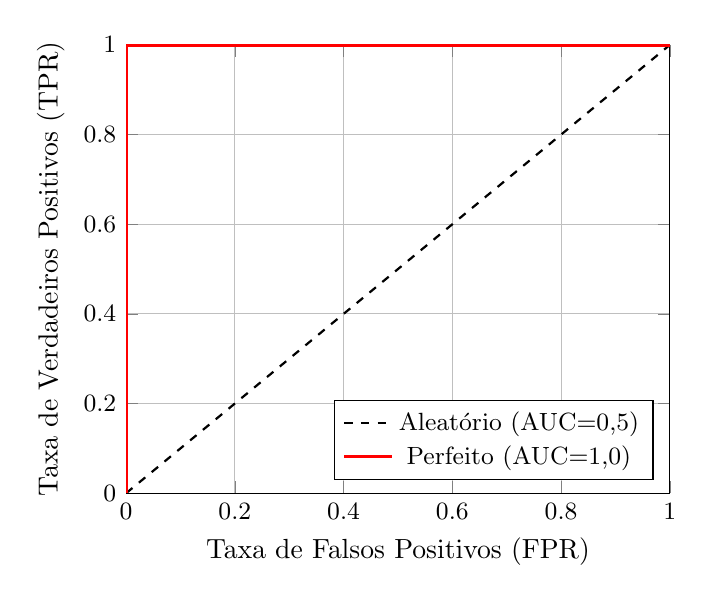
\begin{tikzpicture}
        \begin{axis}[
            width=0.7\textwidth,
            height=0.6\textwidth,
            grid=both,
            xlabel={Taxa de Falsos Positivos (FPR)},
            ylabel={Taxa de Verdadeiros Positivos (TPR)},
            xmin=0, xmax=1,
            ymin=0, ymax=1,
            legend pos=south east,
            legend style={font=\small},
            tick label style={font=\small}
        ]

        % Linha do classificador aleatório
        \addplot[domain=0:1, dashed, thick, color=black] {x};
        \addlegendentry{Aleatório (AUC=0,5)}

        % Curva ROC do Classificador Perfeito
        \addplot[color=red, very thick] coordinates {
            (0,0)  % Inicia
            (0,1)  % Sobe verticalmente até TPR=1, mantendo FPR=0
            (1,1)  % Segue horizontalmente até o fim, mantendo TPR=1
        };
        \addlegendentry{Perfeito (AUC=1,0)}

        \end{axis}
        
    \end{tikzpicture}
    \label{fig:roc_perfect}
    \legend{Fonte: Elaborado pelo autor.}
\end{figure}

A curva vermelha representa um classificador perfeito com TPR, sinônimo de \textit{recall}, sempre igual a um. O raciocínio é que 
para aumentar o \textit{recall}, a quantidade de classes negativas que são classificadas como positivas, calculada por FPR, aumenta. 
Entretanto, para um classificador perfeito, esse \textit{trade-off} não existe.

A linha tracejada representa um classificador aleatório, o \textit{baseline}. Neste caso, por exemplo, para achar 60\% das classes positivas,
cerca de 0,6 de \textit{recall}, o modelo classificaria 60\%  das classes negativas como positivas.

Já a curva PR, Precisão vs \textit{Recall} representa a precisão em função do \textit{recall}. Na figura Figure~\ref{fig:roc_perfect},
é ilustrada a curva PR de um classificador perfeito.

\pgfplotsset{compat=1.18}

\begin{figure}[H]
    \centering
    \caption{Curva Precisão–Recall de um Classificador Perfeito: Comparação com Baseline.}
    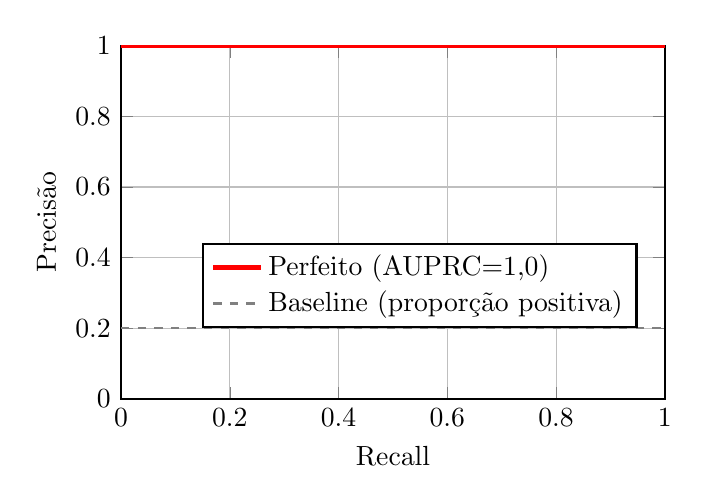
\begin{tikzpicture}
        \begin{axis}[
            width=0.7\textwidth,
            height=0.5\textwidth,
            xlabel={Recall},
            ylabel={Precisão},
            xmin=0, xmax=1,
            ymin=0, ymax=1,
            grid=major,
            legend style={at={(0.95,0.2)},anchor=south east},
            legend cell align={left},
            thick
        ]
        
        % Curva PR do Classificador Perfeito
        \addplot[color=red, ultra thick] coordinates {
            (0.0, 1.0)  % Precisão = 1, Recall = 0
            (1.0, 1.0)  % Precisão = 1, Recall = 1
        };
        \addlegendentry{Perfeito (AUPRC=1,0)}

        % Linha base (baseline) - Mantida como exemplo
        \addplot[dashed, color=gray] coordinates {
            (0,0.2) (1,0.2)
        };
        \addlegendentry{Baseline (proporção positiva)}
        \end{axis}
    \end{tikzpicture}
    
    \label{fig:pr_curve_perfect}
    \legend{Fonte: Elaborado pelo autor.}
\end{figure}

Como há uma relação de \textit{trade-off} entre a precisão e o \textit{recall}, conforme ajusta-se o limiar de decisão para aumentar o \textit{recall},
a precisão tende a cair. Entretanto, assim como ocorre na ROC, esse \textit{trade-off} não existe para um classificador perfeito; ou seja, a precisão é 
sempre 100\% independente do valor do \textit{recall}.

Já a linha tracejada, marca o desempenho de um classificador aleatório; o \textit{baseline}. A linha corresponde a frequência da classe positiva, isto é, 
o classificador aleatório sempre tem uma precisão igual a frequência da classe positiva. AP é o análogo da AUC para esta curva.

Na tabela \ref{tab:matriz_confusao} é ilustrada a matriz de confusão.

\begin{table}[H]
\centering
\caption{Exemplo de matriz de confusão binária}
\label{tab:matriz_confusao}
\begin{tabular}{|c|c|c|}
\hline
\multirow{2}{*}{\textbf{Classe Verdadeira}} & \multicolumn{2}{c|}{\textbf{Classe Predita}} \\ \cline{2-3} 
 & Positiva & Negativa \\ \hline
Positiva & TP & FN \\ \hline
Negativa & FP & TN \\ \hline
\end{tabular}
\legend{Fonte: Elaborado pelo autor.}
\end{table}

Em sentido anti-horário, a partir do canto superior esquerdo temos: 

\begin{enumerate}
\item {TP} \textit{true positive}, quantos casos positivos foram corretamente classificados;
\item {FN} \textit{false negative}, quantos casos positivos foram incorretamente classificados;
\item {FP} \textit{false positive}, quantos casos negativos foram incorretamente classificados;
\item {TN} \textit{true negative}, quantos casos negativos foram incorretamente classificados.
\end{enumerate}

Essas métricas mostram o desempenho do modelo em perspectivas diferentes, 
precisão, \textit{recall}, \textit{f1 score} e acurácia, mostram o desempenho do modelo para um determinado limiar. Neste trabalho, foi escolhido como 50\%. 
Já as curvas PR e ROC mostram o impacto no desempenho do modelo para diferentes limiares e a matriz de confusão permite visualizar os tipos de erros e acertos
individualmente. 

\section{Tipos de redes usadas}
\label{sec:tipo_redes}

Inicialmente, foram escolhidas redes neurais recorrentes (RNNs) e seus subtipos, como LSTM e GRU. Segundo \citeonline{james2023}, esse tipo de rede apresenta grande potencial para lidar com dados sequenciais, como no processamento de linguagem natural, previsão de preços e outros tipos de séries temporais. Como o componente temporal é relevante para o diagnóstico das arritmias, optou-se por esse tipo de modelo.

Além das RNNs, foram utilizadas redes neurais convolucionais (CNNs), conhecidas por sua habilidade em reconhecer padrões em diferentes domínios \citeonline{james2023}. Em particular, CNNs unidimensionais (1D-CNNs) têm se mostrado eficazes na análise de sinais fisiológicos, sendo amplamente aplicadas à classificação de ECG \cite{narotamo2024}.

A motivação para essa combinação está na complementaridade entre os modelos: enquanto as RNNs são eficazes na captura de dependências temporais, as CNNs se destacam na identificação de características morfológicas do sinal.
